\begin{figure}[ht]
	\centering
	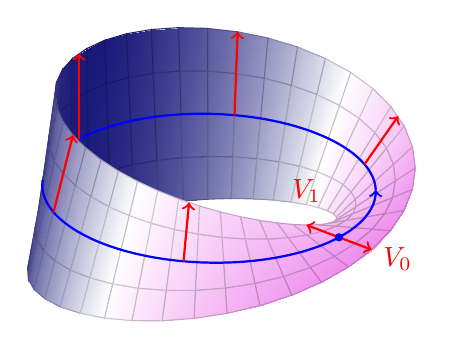
\begin{tikzpicture}
		\begin{axis}[
			hide axis,
			view={40}{40}
			]
			\addplot3 [
			surf, shader=faceted interp,
			point meta=x,
			colormap/violet,
			samples=40,
			samples y=5,
			z buffer=sort,
			domain=0:360,
			y domain=-0.5:0.5
			] (
			{(1+0.5*y*cos(x/2)))*cos(x)},
			{(1+0.5*y*cos(x/2)))*sin(x)},
			{0.5*y*sin(x/2)});
			
			\addplot3 [
			samples=50,
			domain=-145:40, 
			samples y=0,
			thick,
			blue,
			->
			] (
			{cos(x)},
			{sin(x)},
			{0});
			
			\addplot3 [
			samples=50,
			domain=40:180, 
			samples y=0,
			thick,
			blue
			] (
			{cos(x)},
			{sin(x)},
			{0});

			\draw[red, thick, ->] (axis cs: {cos(0)},{sin(0)},{0}) -- (axis cs: {(1+0.5*0.5*cos(0)))*cos(0)},
			{(1+0.5*0.5*cos(0))*sin(0)},
			{0.5*0.5*sin(0)});
			
			\draw[red, thick, ->] (axis cs: {cos(360/6)},{sin(360/6)},{0}) -- (axis cs: {(1+0.5*0.5*cos(360/(2*6)))*cos(360/6)},
			{(1+0.5*0.5*cos(360/(2*6)))*sin(360/6)},
			{0.5*0.5*sin(360/(2*6))});
			
			\draw[red, thick, ->] (axis cs: {cos(2*360/6)},{sin(2*360/6)},{0}) -- (axis cs: {(1+0.5*0.5*cos(2*360/(2*6)))*cos(2*360/6)},
			{(1+0.5*0.5*cos(2*360/(2*6)))*sin(2*360/6)},
			{0.5*0.5*sin(2*360/(2*6))});
			
			\draw[red, thick, ->] (axis cs: {cos(3*360/6)},{sin(3*360/6)},{0}) -- (axis cs: {(1+0.5*0.5*cos(3*360/(2*6)))*cos(3*360/6)},
			{(1+0.5*0.5*cos(3*360/(2*6)))*sin(3*360/6)},
			{0.5*0.5*sin(3*360/(2*6))});
			
			\draw[red, thick, ->] (axis cs: {cos(4*360/6)},{sin(4*360/6)},{0}) -- (axis cs: {(1+0.5*0.5*cos(4*360/(2*6)))*cos(4*360/6)},
			{(1+0.5*0.5*cos(4*360/(2*6)))*sin(4*360/6)},
			{0.5*0.5*sin(4*360/(2*6))});
			
			\draw[red, thick, ->] (axis cs: {cos(5*360/6)},{sin(5*360/6)},{0}) -- (axis cs: {(1+0.5*0.5*cos(5*360/(2*6)))*cos(5*360/6)},
			{(1+0.5*0.5*cos(5*360/(2*6)))*sin(5*360/6)},
			{0.5*0.5*sin(5*360/(2*6))});
			
			\draw[red, thick, ->] (axis cs: {cos(6*360/6)},{sin(6*360/6)},{0}) -- (axis cs: {(1+0.5*0.5*cos(6*360/(2*6)))*cos(6*360/6)},
			{(1+0.5*0.5*cos(6*360/(2*6)))*sin(6*360/6)},
			{0.5*0.5*sin(6*360/(2*6))});
			
			\fill[blue] (axis cs: {1},{0},{0}) circle (1.5pt);
			
			\node[red] at (axis cs: {(1+0.5*0.5*cos(0)))*cos(0)+0.2},
			{(1+0.5*0.5*cos(0))*sin(0)},
			{0.5*0.5*sin(0)}){\(V_0\)};
			\node[red] at (axis cs: {(1-0.5*0.5*cos(0)))*cos(0)},
			{(1-0.5*0.5*cos(0))*sin(0)},
			{-0.5*0.5*sin(0)+0.1}){\(V_1\)};
			
		\end{axis}
					

		
		
	\end{tikzpicture}
	
	\caption{Si prenda come varietà il nastro di M\"obius (come sottovoarietà di \(\R^3\), cf. Sezione~\ref{sez: sottovarietà}) e si consideri la curva \(\gamma\) in blu. In rosso il campo \(V\), ottenuto trasportando parallelemanete \(V_0\). Si osservi che \(V_1 \neq V_0\). }
	
	\label{fig: trasporto parallelo mobius}
\end{figure}